\documentclass{stdlocal}
\begin{document}
\section{Introduction} % (fold)
\label{sec:introduction}

% Nowadays, the majority of application domains vital to the life of humanity is supported by computer-aided systems.
% These are typically programs that provide a set of tools to facilitate the automatic generation, transfer, manipulation, and visualization of domain-specific data by keeping user interaction at a required minimum.
% Computer systems have enabled humanity to streamline processes and to abstract and encapsulate low-level tasks.
% As a consequence, this resulted in the ability to solve harder problems even more efficiently.
% Ironically, these complex automatic systems consisting of multiple layers of abstraction are driven by many processes that might naively be considered rather insignificant.

% Especially
In the area of medicine, examples such as the resection of liver tumors for long-term survival \autocite{alirr2019} and osteotomy planning \autocite{zachow2003} (see figure~\ref{fig:introduction-examples-zachow2003}), that involves reshaping and realigning bones to repair or fix bone-specific issues, show that the use of computer-aided systems for surgery planning reduces the duration of treatment and heavily increases the chance of long-term survival.
Both of the named medical applications simply use curves on the two-dimensional reconstructed surface of scanned medical objects to represent and visualize surgery cuts.
The reconstructed surfaces will thereby be provided as triangular meshes and are often referred to as surface meshes.
As curves on surface meshes are in general a basic building block for tasks involving mesh processing and segmentation \autocite{ji2006,kaplansky2009} (see figures~\ref{fig:introduction-examples-lee2004} and~\ref{fig:introduction-examples-ji2006}), they also play a fundamental role in the areas of computer-aided geometric design, computer graphics, and visualization.
Building on these research areas, significant applications can not only be found in the medical context but also for machine learning \autocite{benhabiles2011,park2019} and engineering.
% \\
% \autocite{zachow2003,alirr2019}

\begin{figure}[b]
  \centering
  \begin{subfigure}[b]{0.32\linewidth}
    \centering
    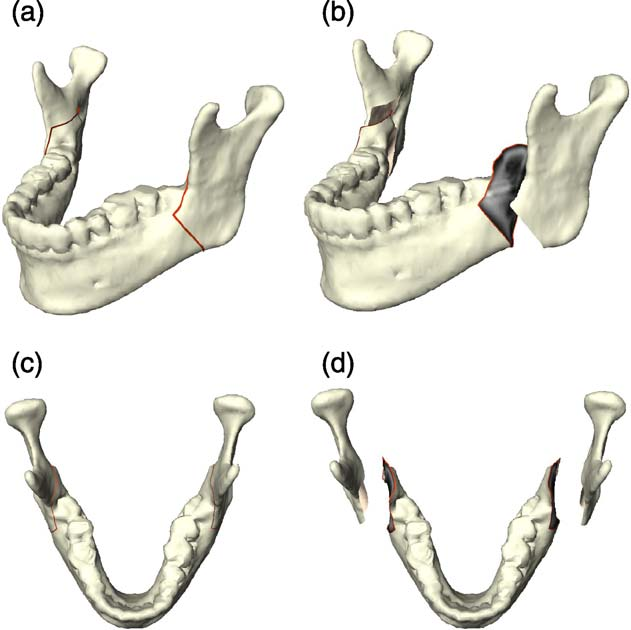
\includegraphics[width=0.75\linewidth,trim={0px 300 340 30},clip]{images/zachow2003-1.png}
    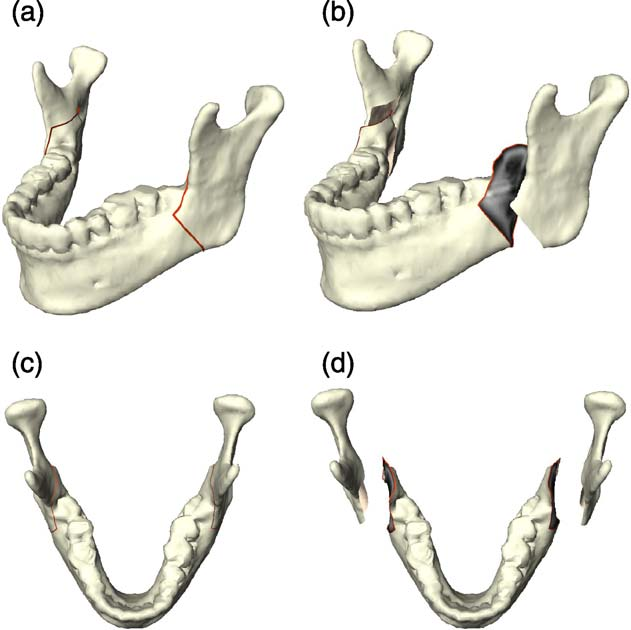
\includegraphics[width=0.75\linewidth,trim={300px 300 0 30},clip]{images/zachow2003-1.png}
    \caption{From \textcite{zachow2003}.}
    \label{fig:introduction-examples-zachow2003}
  \end{subfigure}
  \hfill
  \begin{subfigure}[b]{0.32\linewidth}
    \centering
    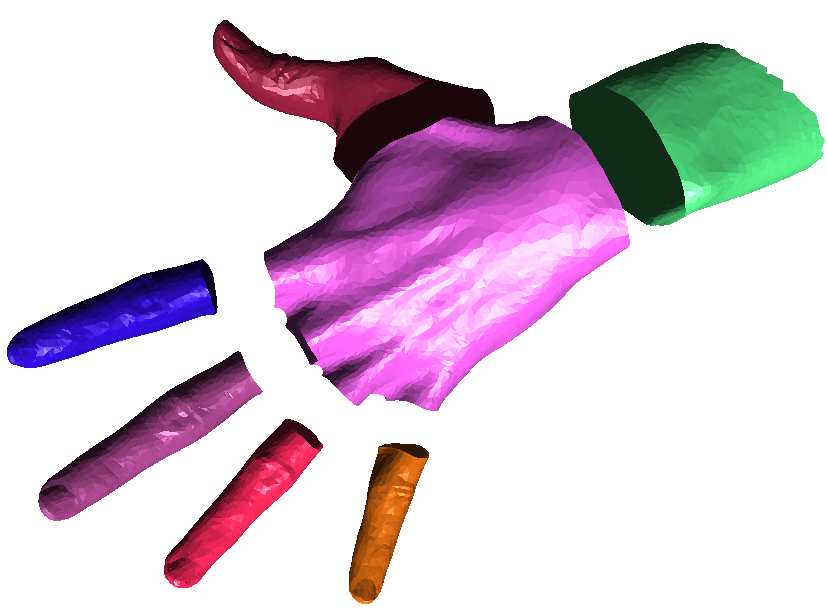
\includegraphics[width=0.85\linewidth]{images/lee2004-1.png}
    \bigskip
    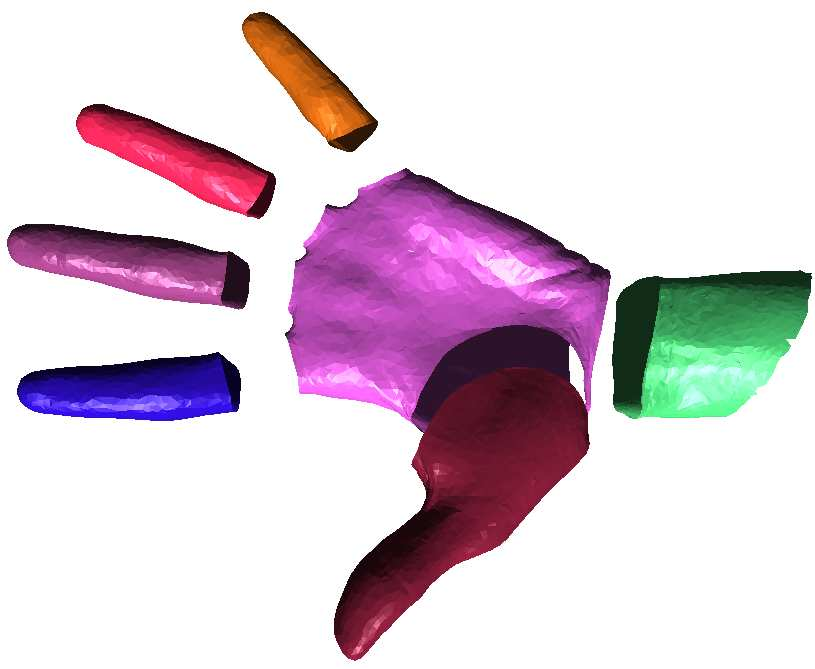
\includegraphics[width=0.85\linewidth]{images/lee2004-2.png}
    \caption{From \textcite{lee2004}.}
    \label{fig:introduction-examples-lee2004}
  \end{subfigure}
  \hfill
  \begin{subfigure}[b]{0.32\linewidth}
    \centering
    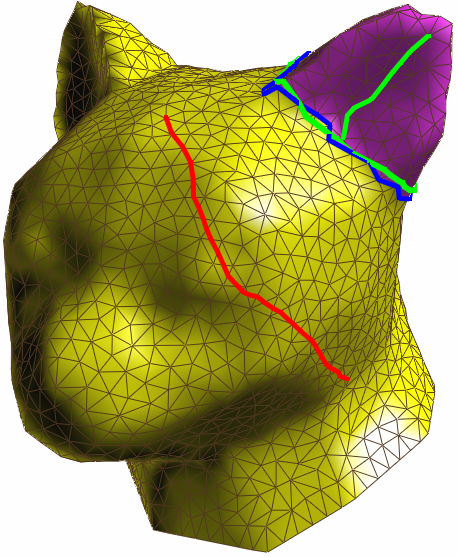
\includegraphics[width=0.6\linewidth]{images/ji2006-1.png}
    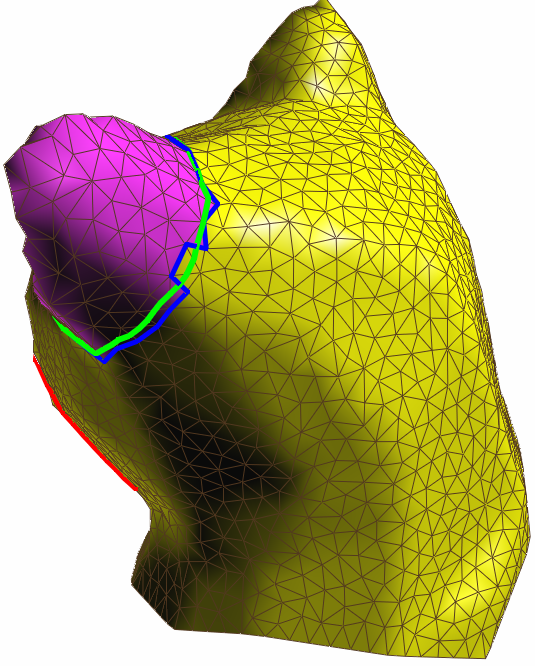
\includegraphics[width=0.6\linewidth]{images/ji2006-2.png}
    \caption{From \textcite{ji2006}.}
    \label{fig:introduction-examples-ji2006}
  \end{subfigure}
  \caption[Application Examples for Smooth Curves on Surface Meshes]{%
    \textbf{Application Examples for Smooth Curves on Surface Meshes}\\
    The images show typical applications for smooth curves on surface meshes, such as osteotomy planning in medicine (left) and surface mesh cutting (middle) and segmentation (right) in computer-aided geometric design and machine learning from other publications.
  }
  \label{fig:introduction-examples}
\end{figure}

Initially chosen curves on surfaces meshes are typically jagged due to the finite precision of the underlying mesh and emit curvature noise that is not neglectable and perceivable by the human eye.
Hence, a smoothing process is applied to reduce their overall curvature and attain surface cuts with well-defined properties.
In general, the result of curve smoothing might strongly deviate from the initially given curve to fulfill the provided constraints.
For medical surface cutting applications, though, the shape of an initial curve is defined by domain experts, such as physicians or bioengineers, and most likely indicates relevant anatomical landmarks or surface regions.
Thus, under these circumstances, the smoothing additionally requires the resulting curve to be close to its original such that no essential information is lost during the process.
\autocite{lawonn2014}\footnote{In this thesis, citations concerning a whole paragraph will be given after the last sentence of the very paragraph.}

% Consequently, their fundamental role in the areas of computer-aided geometric design, computer graphics, and visualization
%, that are heavily based on mesh processing,
% is unconcealable.
% So, curve smoothing on surface meshes is not only relevant in specific areas of medicine but is a generally applicable and important tool to many other domains of applications building on the above research areas.
% Further domain areas, such as machine learning \autocite{benhabiles2011,park2019} and engineering, therefore provide many more direct and significant applications.

Besides their mathematical correctness and convergence, curve smoothing algorithms should exhibit a certain level of adaptivity with respect to the given surface mesh and its initially chosen curve.
Surface meshes are most typically an irregular grid of triangular faces that may highly vary in diameter and area.
In addition, the initial curve might be extreme concerning its length, curvature, and overall shape.
An algorithm to smooth curves on surface meshes needs to adapt to all these situations and still figure out the best possible result that abides to the given criteria.
In conjunction with its correctness, this also means that such an algorithm needs to be robust for many different kinds of scenarios, such as self-intersecting curves and noisy surface geometries.
% , that may result in wrong calculations based on the finite precision of floating-point values.
Yet another property to take into account is the efficiency of the algorithm.
To seamlessly integrate curve smoothing into the user interface of a computer-assisted system for domain-specific applications, it at least needs to provide an interactive up to real-time performance.
As a consequence, the implementation and application programming interface (API) design of such algorithms is assumed to be an involved task and error-prone and should not be handled by a custom implementation for each framework. \\
%when the programmer intends to apply the algorithm on a wide variety of cases.
\autocite{lawonn2014}

% There are a few already existing algorithms for producing smoothed curves on surface meshes \autocite{hofer2004,martinez2007,lawonn2014,mancinelli2022}.
Previous solutions to these problems involving the use of energy-minimizing splines \autocite{hofer2004} and generalizations of Bézier splines to three-dimensional surfaces \autocite{martinez2007,mancinelli2022}, while offering a general approach and sophisticated tools, either suffer from poor performance and numerical instabilities or are not sufficient for applications in a medical context.
Using an iterative method that is based on the reduction of local geodesic curvature, \textcite{lawonn2014} were able to construct a robust curve smoothing algorithm which preserves closeness to the initial curve.
They successfully applied it to the decomposition of cerebral aneurysms and the resection planning for liver surgery.
Unfortunately, the initial selection and propagation of desired curvature values when handling critical or splitting vertices is not provided or at least inconsistent.

% All the above references define their algorithm and explain its properties in great detail.
% For the above methods, programming procedures were provided as pseudocode and quality in comparison to similar algorithms has been evaluated
The above publications compare the quality of generated curves to alternative algorithms and describe the algorithm's programming procedures with respect to a high-level point of view.
% based on pseudocode.
However, the very low-level details about the composition of data structures, advice for an implementation in a specific programming language, or ways to handle difficult corner cases are typically left out.
This makes the comparison of the performance and robustness of algorithms much harder and unreproducible.
%, because custom implementations would need to be used.
Furthermore, there is no widely accepted metric to compare the smoothness of two given curves which leads to a highly subjective treatment and evaluation of different smoothing algorithms.

For the implementation of curve smoothing algorithms that allow for high-performance, reproducibility, and robustness, adequate candidates would be the modern standards of the C++ programming language in conjunction with the OpenGL graphics API.
C++ is a multi-paradigm language that integrates many different programming styles, such as object-oriented, functional, and data-oriented programming.
It is still the de-facto standard for graphics applications and well-known to be one of the fastest languages in the world which incorporates low-level programming facilities, such as inline assembly, and efficient high-level abstraction mechanisms, like template meta programming.
% The design of the whole language keeps on advancing to make programs faster and easier to develop.
% In the most common cases, C++ can be seen as a superset of the older C programming language which is typically used by other programming languages to provide the possibility of code being called from different languages.
% Therefore the users of the framework are not even restricted to use C++ but instead are able to use other languages, like Python, to communicate with a C interface to achieve similar results.
OpenGL is the open-source graphics API that allows programs to efficiently communicate and interact with the driver of the graphics card to visualize given data.
Through the use of so-called compute shaders, written code is able to run concurrently on the GPU independently of the graphics card's manufacturer or the operating system.
% By using them, no strong constraints are imposed on the software environment that the software framework is running on.
% Both tools allow for a sophisticated modularization of the whole framework.
% So, no user needs to pay for features that are not needed.
\autocite{stroustrup2014,meyers2014,vandevoorde2018,reddy2011,cppreference,isocpp,opengl}

% In this thesis, precisely in sections \ref{sec:design} and \ref{sec:implementation}, we develop a new library and program, called \citetitle{nanoreflex}\footfullcite{nanoreflex}, using the C++ programming language in conjunction with the OpenGL graphics API.
In this thesis, precisely in sections \ref{sec:design} and \ref{sec:implementation}, a robust and efficient algorithm, called \citetitle{nanoreflex}\footfullcite{nanoreflex}, to smooth discrete curves on triangular surface meshes is developed using the C++ programming language in conjunction with the OpenGL graphics API.
The method described here is based on the work of \textcite{lawonn2014} which seems to be the most promising approach for medical purposes.
It improves their initial selection and propagation of desired curvatures by using weighted stencils and curvature textures.
Incorporating efficient data structures and heuristics shown to work by \textcite{mancinelli2022}, \citetitle{nanoreflex} implements parallelized versions on the CPU and GPU which should be applicable in a wide variety of cases.
% Hereby, a special emphasis lies on the design for medical purposes.
The source code is provided as an open-source repository on GitHub.
% It is easily installable on every operating system.
The necessary theoretical background to understand the design- and the implementation-specific aspects is given in section~\ref{sec:preliminaries}.
Here, we will give a brief introduction to differential geometry and polyhedral manifolds.
A mathematical rigorous discussion about the algorithm will be part of section~\ref{sec:design} to properly encapsulate all the information specific to the implementations.
Section~\ref{sec:previous_work} refers to some related work concerning general curves, geodesics and the smoothing of curves on surfaces.
Afterwards, in section~\ref{sec:application}, \citetitle{nanoreflex} is applied to the segmentation of lung lobes \autocite{park2019}.
In section~\ref{sec:evaluation}, the algorithm will be used on the \citetitle{thingi10k} dataset and other test cases to evaluate its robustness and efficiency.
At the end, in section~\ref{sec:conclusions}, I will give a brief summary of the thesis and a discussion dealing with advantages, disadvantages, and further improvements.

% section introduction (end)
\end{document}
